\section{Definição}

\begin{frame}[fragile]{Listas duplamente encadeadas}

    \begin{itemize}
        \item Uma lista duplamente encadeada é uma estrutura composta por nós,
            onde cada nó armazenada uma informação, um ponteiro para o antecessor e um 
            ponteiro para o próximo nó da lista

        \item A partir de qualquer elemento da lista é possível acessar todos os demais elementos

        \item Esta maior flexibilidade em relação às listas (simplesmente) encadeadas tem
            seu custo: cada nó precisa de um ponteiro extra, aumentando o uso de memória

        \item É uma estrutura de dados linear, devido a travessia sequencial e ordenada
            de seus elementos

        \item Por conta da estrutura dos nós, o acesso aleatório em listas duplamente encadeadas 
            tem complexidade $O(N)$

    \end{itemize}

\end{frame}

\begin{frame}[fragile]{Visualização de uma lista duplamente encadeada}

    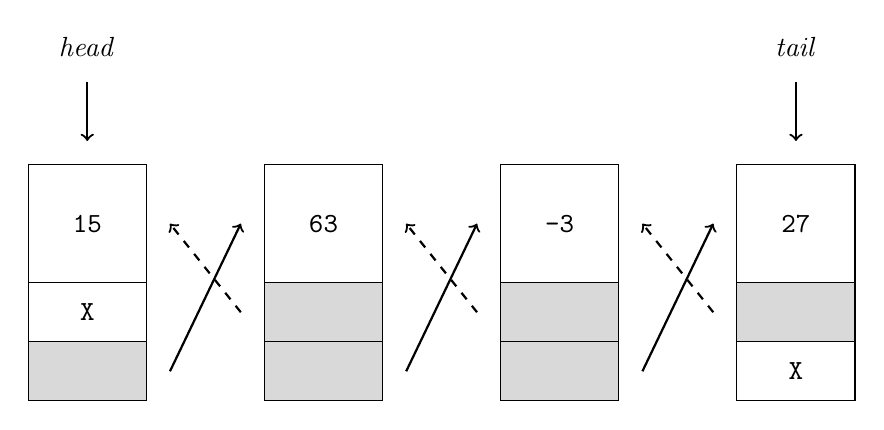
\begin{tikzpicture}[scale=1.5]
        \node[anchor=center] at (0.5, 3) {\textit{head}};
        \draw[->,thick] (0.5, 2.7) -- (0.5, 2.2);

        \node[anchor=center] at (6.5, 3) {\textit{tail}};
        \draw[->,thick] (6.5, 2.7) -- (6.5, 2.2);

        \draw[fill=white] (0,1) rectangle (1,2);
        \node at (0.5,0.75) {\textbf{\texttt{X}}};
        \draw (0,0.5) rectangle (1,1);
        \draw[fill=gray!30] (0,0) rectangle (1,0.5);
        \node at (0.5,1.5) {\texttt{15}};

        \draw[->,thick] (1.2, 0.25) -- (1.8, 1.5);
        \draw[->,thick,dashed] (1.8, 0.75) -- (1.2, 1.5);

        \draw[fill=white] (2,1) rectangle (3,2);
        \draw[fill=gray!30] (2,0) rectangle (3,0.5);
        \draw[fill=gray!30] (2,0.5) rectangle (3,1);
        \node at (2.5,1.5) {\texttt{63}};

        \draw[->,thick] (3.2, 0.25) -- (3.8, 1.5);
        \draw[->,thick,dashed] (3.8, 0.75) -- (3.2, 1.5);

        \draw[fill=white] (4,1) rectangle (5,2);
        \draw[fill=gray!30] (4,0) rectangle (5,0.5);
        \draw[fill=gray!30] (4,0.5) rectangle (5,1);
        \node at (4.5,1.5) {\texttt{-3}};

        \draw[->,thick] (5.2, 0.25) -- (5.8, 1.5);
        \draw[->,thick,dashed] (5.8, 0.75) -- (5.2, 1.5);

        \draw[fill=white] (6,1) rectangle (7,2);
        \draw (6,0) rectangle (7,0.5);
        \draw[fill=gray!30] (6,0.5) rectangle (7,1);
        \node at (6.5,1.5) {\texttt{27}};
        \node at (6.5,0.25) {\textbf{\texttt{X}}};

    \end{tikzpicture}

\end{frame}

\begin{frame}[fragile]{Implementação de uma lista duplamente encadeada}

    \begin{itemize}
        \item Uma lista duplamente encadeada pode ser implementada como uma \code{c}{struct} em C 
            ou uma classe em C++

        \item Ela deve ter um membro para o primeiro (\textit{head}) e para o último
            (\textit{tail}) elemento da lista

        \item Cada nó deve ter, no mínimo, três membros: um para armazenar as informações 
            (\code{c}{info}), um para representar o ponteito para o próximo nó
            (\code{c}{next}) e um para representar o ponteiro para o nó anterior
            (\code{c}{prev})

        \item O primeiro elemento da lista tem membro \code{c}{prev} nulo
        \item O último elemento da lista tem membro \code{c}{next} nulo

        \item Esta configuração permite inserções e remoções, no íncio e no final, com
            complexidade $O(1)$
    \end{itemize}

\end{frame}

\begin{frame}[fragile]{Exemplo de implementação de uma lista duplamente encadeada}
    \inputsnippet{cpp}{1}{20}{list.h}
\end{frame}

\begin{frame}[fragile]{Exemplo de implementação de uma lista duplamente encadeada}
    \inputsnippet{cpp}{21}{40}{list.h}
\end{frame}

\begin{frame}[fragile]{Exemplo de implementação de uma lista duplamente encadeada}
    \inputsnippet{cpp}{90}{110}{list.h}
\end{frame}

